\documentclass[11pt,a4paper]{article}

% --- packages ---
\usepackage[margin=0.95in,headheight=15pt]{geometry}
\usepackage{graphicx}
\usepackage{amsmath, amssymb}
\usepackage{booktabs}
\usepackage{array}
\usepackage{xcolor}
\usepackage{hyperref}
\usepackage{caption}
\usepackage{subcaption}
\usepackage{float}
\usepackage{enumitem}
\usepackage{fontenc}
\usepackage{inputenc}
\usepackage{titlesec}
\usepackage{parskip}
\usepackage{fancyhdr}
\usepackage{tabularx}
\usepackage{colortbl}
\usepackage{mdframed}

% --- colors ---
\definecolor{iitjblue}{RGB}{0, 56, 101}
\definecolor{accentblue}{RGB}{30, 120, 190}
\definecolor{lightgray}{RGB}{245, 245, 245}
\definecolor{darkgray}{RGB}{60, 60, 60}
\definecolor{green}{RGB}{34, 139, 34}
\definecolor{red}{RGB}{178, 34, 34}

% --- hyperlinks ---
\hypersetup{
    colorlinks=true,
    linkcolor=accentblue,
    citecolor=accentblue,
    urlcolor=accentblue,
}

% --- section formatting ---
\titleformat{\section}
  {\Large\bfseries\color{iitjblue}}
  {\thesection.}{0.5em}{}[\titlerule]

\titleformat{\subsection}
  {\large\bfseries\color{accentblue}}
  {\thesubsection.}{0.5em}{}

\titleformat{\subsubsection}
  {\normalsize\bfseries\color{darkgray}}
  {\thesubsubsection.}{0.5em}{}

% --- header / footer ---
\pagestyle{fancy}
\fancyhf{}
\lhead{\textcolor{iitjblue}{\footnotesize Problem 1}}
\rhead{\textcolor{iitjblue}{\footnotesize B23CM1054}}
\cfoot{\thepage}
\renewcommand{\headrulewidth}{0.4pt}

% --- highlight box ---
\newmdenv[
  backgroundcolor=lightgray,
  linecolor=accentblue,
  linewidth=1.5pt,
  topline=false, bottomline=false,
  rightline=false,
  leftmargin=5pt, rightmargin=5pt,
  innerleftmargin=10pt,
  innertopmargin=6pt, innerbottommargin=6pt,
]{notebox}

% =========================================
\begin{document}

% --- title page ---
\begin{titlepage}
  \centering
  \vspace*{2cm}
  {\color{iitjblue}\rule{\linewidth}{2pt}}\vspace{0.4cm}

  {\Huge\bfseries\color{iitjblue} Natural Language Understanding\\[0.3em]
   \Large Assignment -- 2}\\[0.6em]

  {\color{iitjblue}\rule{\linewidth}{2pt}}

  \vspace{1.5cm}
  {\Large\bfseries Problem 1}\\[2em]

  \vfill
  \textit{\color{darkgray}
    Word2Vec models trained on text scraped from iitj.ac.in\\
    using CBOW and Skip-gram with Negative Sampling.}
  \vspace{1cm}
\end{titlepage}

% --- table of contents ---
\tableofcontents
\newpage

% =========================================
\section{Introduction}
% =========================================

The idea here is pretty straightforward --- grab a bunch of text from the IIT Jodhpur website, train Word2Vec models on it, and then check if the word vectors actually make sense for terms you'd expect on a university website (\textit{research}, \textit{phd}, \textit{student}, \textit{exam}, etc.).

We train two kinds of Word2Vec models:
\begin{itemize}[nosep]
  \item \textbf{CBOW} --- predicts the middle word from the surrounding context words.
  \item \textbf{Skip-gram with Negative Sampling (SGNS)} --- does the reverse, predicts context from the middle word.
\end{itemize}

Three configs each (different dimensions, window sizes, negative samples) gives us six models total. We train all six \textbf{both} with gensim (the standard library) \textbf{and} with a from-scratch numpy implementation, then compare the two approaches. After that we look at nearest neighbours, try some analogy tasks, and visualize it all with PCA and t-SNE.

% =========================================
\section{Dataset Preparation}
% =========================================

\subsection{Data Collection}

We scraped text from \texttt{iitj.ac.in} using Python (\texttt{requests} + \texttt{BeautifulSoup} for HTML pages, \texttt{PyMuPDF} for PDFs). The scraper does a BFS crawl starting from around 110 hand-picked seed URLs covering all the major sections of the website.

\begin{enumerate}[leftmargin=2em, label=\arabic*.]
  \item \textbf{250 web pages} --- departments (CSE, EE, ME, Civil, Chemical, etc.), schools (AI\&DS, Design, Liberal Arts, Management), offices (academics, R\&D, placements, director), labs (CRF, DIA), admissions, news, announcements.
  \item \textbf{Academic Regulations PDFs} --- UG regs (2019), PG regs (2022), M.S.\ by Research (2023). These alone gave us a ton of semester/credit/grade/thesis vocabulary.
  \item \textbf{Annual Reports} --- from 2008--09 through 2023--24 (8 reports). Big source of research, infrastructure, and achievement data.
  \item \textbf{IIT Act \& Statutes} --- the original 1961 Act, 2012 Amendment, and IITJ First Statutes.
  \item \textbf{NIRF Reports} --- 2025 Overall and Engineering rankings data.
  \item \textbf{Other stuff} --- IPR policy, R\&D norms, placement brochure, department brochures, sponsored research docs.
\end{enumerate}

Hindi pages were filtered out (any URL with \texttt{/hi/} gets skipped), and PDFs go through an English-detection check before being kept.

\subsection{Preprocessing Pipeline}

The raw text goes through these cleaning steps before training:

\begin{enumerate}[leftmargin=2em, label=\Roman*.]
  \item \textbf{URL \& email removal} --- regex-based.
  \item \textbf{HTML tag removal} --- strip \texttt{<script>}, \texttt{<nav>}, \texttt{<footer>}, leftover tags.
  \item \textbf{Non-ASCII removal} --- only printable ASCII kept (removes Hindi that slipped through).
  \item \textbf{Sentence splitting} --- via \texttt{nltk.sent\_tokenize}.
  \item \textbf{Tokenization \& lowercasing} --- \texttt{word\_tokenize}, then lowercase.
  \item \textbf{Stopword removal} --- NLTK English stopwords + domain noise (\textit{iitj, www, html, login}, etc.).
  \item \textbf{Length filter} --- tokens under 3 characters dropped; sentences under 3 tokens dropped.
\end{enumerate}

\subsection{Dataset Statistics}

\begin{notebox}
\textbf{Raw corpus:} 51 files, \textbf{\textasciitilde809K words} total.\\[0.3em]
\textbf{After preprocessing:} \textbf{26,123 sentences}, \textbf{450,793 tokens}, vocabulary of \textbf{27,241 unique words}.\\[0.3em]
After \texttt{min\_count=2} filtering during training $\to$ \textbf{16,990 words} in model vocabulary.
\end{notebox}

\subsection{Word Cloud}

Figure~\ref{fig:wordcloud} shows the most common words in the corpus. Dominant terms like \textit{engineering}, \textit{technology}, \textit{research}, \textit{institute} clearly reflect IITJ's academic identity.

\begin{figure}[H]
  \centering
  
\includegraphics[width=0.9\linewidth]{outputs/wordcloud.png}
  \caption{Word cloud of the cleaned IITJ corpus. Size = frequency.}
  \label{fig:wordcloud}
\end{figure}

% =========================================
\section{Word2Vec Models}
% =========================================

\subsection{Theory}

\subsubsection{CBOW}

CBOW predicts a target word $w_t$ from its surrounding context. Given window size $c$, the context is $\mathcal{C} = \{w_{t-c},\ldots,w_{t-1},w_{t+1},\ldots,w_{t+c}\}$. The model averages context embeddings and passes through softmax:
\[
  \hat{v} = \frac{1}{2c}\sum_{-c \le j \le c,\, j \ne 0} \mathbf{v}_{w_{t+j}} \qquad
  P(w_t \mid \mathcal{C}) = \frac{\exp(\mathbf{u}_{w_t}^\top \hat{v})}{\sum_{w \in V} \exp(\mathbf{u}_w^\top \hat{v})}
\]

CBOW trains fast and gives smoother representations, especially for frequent words.

\subsubsection{Skip-gram with Negative Sampling}

Skip-gram does the inverse --- given center word $w_t$, predict each context word. \textbf{Negative sampling} replaces the expensive full softmax with a binary classifier that distinguishes real context from $k$ noise words:
\[
  \mathcal{L}_{\text{NS}} = \log \sigma(\mathbf{u}_{w_O}^\top \mathbf{v}_{w_I})
  + \sum_{i=1}^{k} \mathbb{E}_{w_i \sim P_n(w)}\!\left[\log \sigma(-\mathbf{u}_{w_i}^\top \mathbf{v}_{w_I})\right]
\]
where $P_n(w) \propto f(w)^{3/4}$ down-weights very common words in the noise distribution. Skip-gram is better at handling rare words and gives sharper semantic distinctions.

\subsubsection{Cosine Similarity \& Analogies}

Similarity is measured with cosine: $\text{sim}(\mathbf{a}, \mathbf{b}) = \frac{\mathbf{a} \cdot \mathbf{b}}{\|\mathbf{a}\|\,\|\mathbf{b}\|}$

Analogies use \textbf{3CosAdd}: for ``$a : b :: c : ?$'', find $w$ closest to $\mathbf{v}_b - \mathbf{v}_a + \mathbf{v}_c$.

\subsection{Hyperparameter Configurations}

We trained three configs per architecture to see the effect of embedding dimension, context window, and negative samples.

\begin{table}[H]
\centering
\caption{Hyperparameter grid for all six trained models.}
\renewcommand{\arraystretch}{1.3}
\rowcolors{2}{lightgray}{white}
\begin{tabularx}{\textwidth}{lcccccX}
\toprule
\textbf{Model} & \textbf{Arch.} & \textbf{Dim} & \textbf{Window} & \textbf{Neg.} & \textbf{Epochs} & \textbf{Time (s)} \\
\midrule
CBOW\_A & CBOW      & 50  & 3 & --  & 15 & 2.90 \\
CBOW\_B & CBOW      & 100 & 5 & --  & 15 & 3.07 \\
CBOW\_C & CBOW      & 200 & 7 & --  & 20 & 4.98 \\
SG\_A   & Skip-gram & 50  & 3 & 5   & 15 & 4.55 \\
SG\_B   & Skip-gram & 100 & 5 & 10  & 15 & 10.14 \\
SG\_C   & Skip-gram & 200 & 7 & 15  & 20 & 32.20 \\
\bottomrule
\end{tabularx}
\label{tab:configs}
\end{table}

All models used \texttt{min\_count=2}, \texttt{workers=4}, \texttt{seed=42}. CBOW uses hierarchical softmax (\texttt{hs=1}), Skip-gram uses negative sampling (\texttt{hs=0}).

\begin{figure}[H]
  \centering
  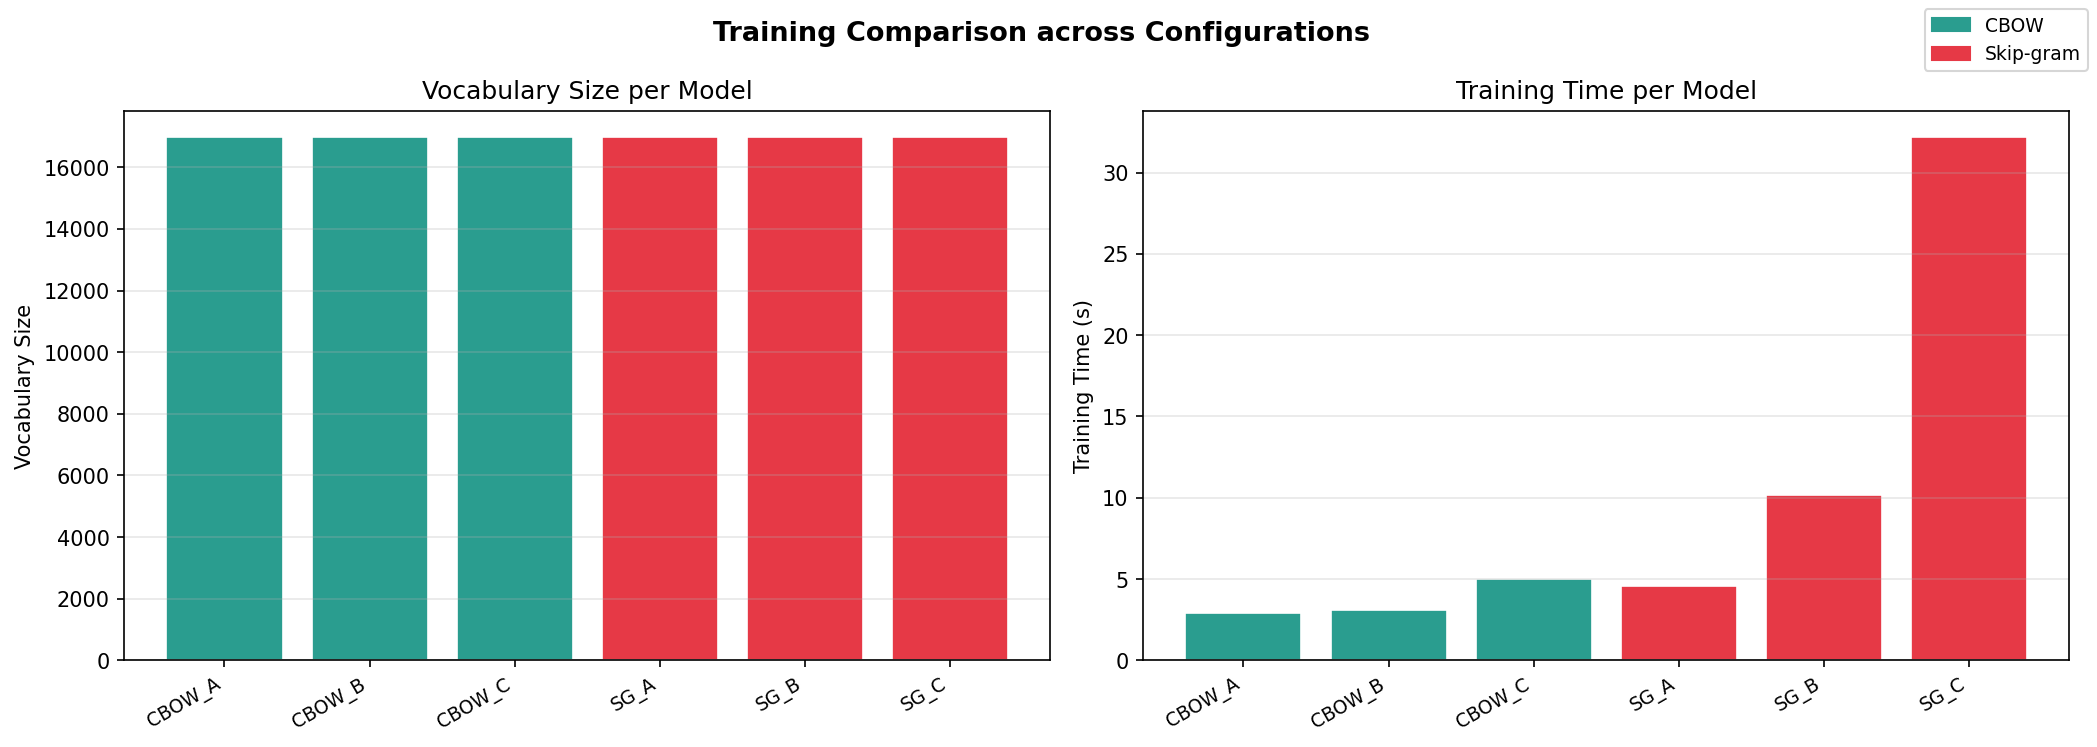
\includegraphics[width=0.92\linewidth]{outputs/training_comparison.png}
  \caption{Vocabulary size (all 16,990) and training time across configs. Skip-gram is slower because it processes each context word independently.}
  \label{fig:training}
\end{figure}

% =========================================
\section{Semantic Analysis}
% =========================================

\subsection{Top-5 Nearest Neighbours}

Table~\ref{tab:nn} shows the five nearest neighbours for four probe words, comparing CBOW\_B and SG\_B (both 100-d, window 5).

\begin{table}[H]
\centering
\caption{Top-5 nearest neighbours. Cosine similarity in parentheses.}
\renewcommand{\arraystretch}{1.35}
\small
\rowcolors{2}{lightgray}{white}
\begin{tabularx}{\textwidth}{lXX}
\toprule
\textbf{Word} & \textbf{CBOW\_B (dim=100, win=5)} & \textbf{SG\_B (dim=100, win=5, neg=10)} \\
\midrule
\texttt{research}
  & projects (0.46), mapped (0.39), drdo (0.39), chemistry (0.37), ongoing (0.35)
  & undertaking (0.65), cant (0.65), signi (0.64), cie (0.64), worthy (0.62) \\
\addlinespace
\texttt{student}
  & students (0.45), scholar (0.40), ordinary (0.39), curricular (0.37), scholars (0.37)
  & rachit (0.55), recipients (0.55), aeromodeling (0.55), ably (0.54), elections (0.54) \\
\addlinespace
\texttt{phd}
  & fellowship (0.55), mmt (0.40), tcs (0.37), scholar (0.36), prestigious (0.36)
  & recipients (0.69), mtech (0.68), lovish (0.68), namanbaghel (0.67), rachit (0.64) \\
\addlinespace
\texttt{exam}
  & thinkers (0.42), tuesday (0.38), commissioned (0.38), examination (0.38), indicon (0.36)
  & syllabus (0.73), qualify (0.71), scripts (0.69), entrance (0.68), screened (0.66) \\
\bottomrule
\end{tabularx}
\label{tab:nn}
\end{table}

\subsubsection*{Discussion}

\begin{notebox}
\textbf{Key takeaway:} Skip-gram is sharper for specific terms (exam $\to$ syllabus, entrance), but also picks up corpus noise (PhD $\to$ student names from award lists). CBOW is more stable but less specific.
\end{notebox}

\begin{itemize}[leftmargin=1.5em]
  \item \textbf{CBOW gives broader associations.} For ``research'' it finds \textit{projects, drdo, chemistry} --- general research-related stuff. For ``student'' it gets \textit{students, scholar, scholars} --- mostly morphological variants.
  \item \textbf{Skip-gram is sharper but noisier.} For ``exam'' it nails it with \textit{syllabus, qualify, entrance, screened} --- very specific exam-related words. But for ``phd'' it picks up student names (\textit{lovish, namanbaghel, rachit}) that appear next to ``PhD'' in annual report award lists. That's a corpus artifact, not a model problem.
  \item \textbf{Overall:} CBOW is stable, SG captures finer distinctions but is more sensitive to data noise.
\end{itemize}

\subsection{Analogy Experiments}

Five analogies tested using 3CosAdd on SG\_B:

\begin{table}[H]
\centering
\caption{Analogy results using SG\_B (dim=100). Top-3 answers shown.}
\renewcommand{\arraystretch}{1.35}
\small
\rowcolors{2}{lightgray}{white}
\begin{tabularx}{\textwidth}{lX}
\toprule
\textbf{Analogy (\textit{a} : \textit{b} :: \textit{c} : ?)} & \textbf{Top Results (cosine)} \\
\midrule
undergraduate : bachelor :: postgraduate : ?
  & icwa (0.60), iti (0.60), applicant (0.56) \\
professor : research :: student : ?
  & worth (0.50), extramural (0.50), indicated (0.49) \\
department : course :: faculty : ?
  & interestunder (0.49), maturity (0.49), anindependent (0.49) \\
examinations : grade :: semester : ?
  & averages (0.49), cutoff (0.49), transcript (0.49) \\
bachelor : undergraduate :: master : ?
  & masters (0.56), bouquet (0.55), graduate (0.54) \\
\bottomrule
\end{tabularx}
\label{tab:analogies}
\end{table}

\subsubsection*{Discussion}

\begin{itemize}[leftmargin=1.5em]
  \item \textbf{Analogy 4 (examinations : grade :: semester : ?)} returns \textit{averages, cutoff, transcript, dgpa}. These are all grade-related terms that naturally follow ``semester'' in academic regulations text. Semantically pretty coherent.
  \item \textbf{Analogy 5 (bachelor : undergraduate :: master : ?)} returns \textit{masters, graduate} --- reasonable answers.
  \item \textbf{Some analogies fail} --- Analogy 3 returns junk like \textit{interestunder} (a PDF parsing artifact where two words got concatenated). That's a data quality issue.
  \item Generally, analogies are harder on domain-specific corpora because the vector space is built around IITJ co-occurrence patterns, not general English.
\end{itemize}

% =========================================
\section{From-Scratch Implementation}
% =========================================

In addition to gensim, we implemented Word2Vec entirely from scratch using only \texttt{numpy} --- no external ML libraries. This lets us understand the internals of the algorithm and compare against an optimized industrial implementation.

\subsection{Implementation Details}

Our scratch implementation covers:

\begin{enumerate}[leftmargin=2em, label=\arabic*.]
  \item \textbf{Vocabulary building} --- frequency counting, \texttt{min\_count} filtering, word-to-index mapping.
  \item \textbf{Subsampling} --- frequent words are randomly dropped with probability $P_{\text{keep}}(w) = \sqrt{t / f(w)}$ where $t = 10^{-5}$ (same as the original Word2Vec paper).
  \item \textbf{Negative sampling distribution} --- $P_n(w) \propto f(w)^{0.75}$ to down-weight very common noise words.
  \item \textbf{CBOW with negative sampling} --- average context embeddings $\to$ dot product with center word $\to$ binary cross-entropy against $k$ noise samples $\to$ SGD update.
  \item \textbf{Skip-gram with negative sampling} --- center word embedding $\to$ dot product with each context word $\to$ same negative sampling loss $\to$ SGD.
  \item \textbf{Linear learning rate decay} --- $\alpha_t = \alpha_0 \cdot (1 - t/T)$, decaying from \texttt{0.05} (CBOW) or \texttt{0.025} (SG) to near zero.
\end{enumerate}

\begin{notebox}
\textbf{Key difference:} Gensim's CBOW uses hierarchical softmax (\texttt{hs=1}), while our scratch CBOW uses negative sampling for both architectures --- hierarchical softmax requires building a Huffman tree, which is complex to implement from scratch.
\end{notebox}

\subsection{Scratch Model Configurations}

Same hyperparameters as the gensim models for a fair comparison:

\begin{table}[H]
\centering
\caption{From-scratch model training summary.}
\renewcommand{\arraystretch}{1.3}
\rowcolors{2}{lightgray}{white}
\begin{tabularx}{\textwidth}{lcccccc}
\toprule
\textbf{Model} & \textbf{Arch.} & \textbf{Dim} & \textbf{Window} & \textbf{Neg.} & \textbf{Epochs} & \textbf{Time (s)} \\
\midrule
CBOW\_A & CBOW      & 50  & 3 & 5  & 15 & 230 \\
CBOW\_B & CBOW      & 100 & 5 & 5  & 15 & 234 \\
CBOW\_C & CBOW      & 200 & 7 & 5  & 20 & 320 \\
SG\_A   & Skip-gram & 50  & 3 & 5  & 15 & 619 \\
SG\_B   & Skip-gram & 100 & 5 & 10 & 15 & 1120 \\
SG\_C   & Skip-gram & 200 & 7 & 15 & 20 & 2276 \\
\bottomrule
\end{tabularx}
\label{tab:scratch_configs}
\end{table}

\subsection{Gensim vs.\ Scratch: Training Speed}

Gensim is written in C with Python bindings, so naturally it's way faster:

\begin{table}[H]
\centering
\caption{Training time comparison. Gensim's C backend is 64--136$\times$ faster.}
\renewcommand{\arraystretch}{1.3}
\rowcolors{2}{lightgray}{white}
\begin{tabularx}{\textwidth}{lrrr}
\toprule
\textbf{Model} & \textbf{Gensim (s)} & \textbf{Scratch (s)} & \textbf{Slowdown} \\
\midrule
CBOW\_A & 2.90  & 230   & 79$\times$ \\
CBOW\_B & 3.07  & 234   & 76$\times$ \\
CBOW\_C & 4.98  & 320   & 64$\times$ \\
SG\_A   & 4.55  & 619   & 136$\times$ \\
SG\_B   & 10.14 & 1120  & 110$\times$ \\
SG\_C   & 32.20 & 2276  & 71$\times$ \\
\bottomrule
\end{tabularx}
\label{tab:time_compare}
\end{table}

\begin{figure}[H]
  \centering
  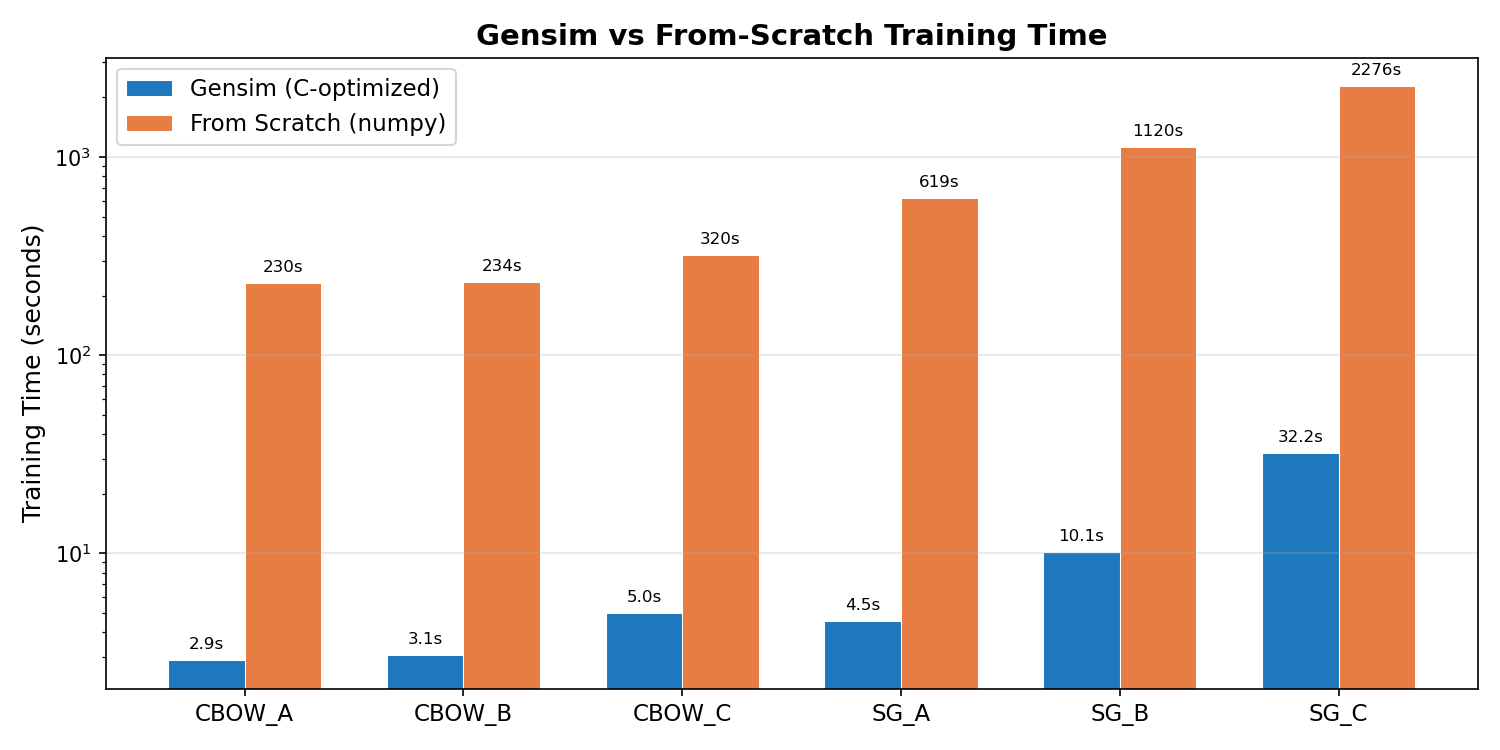
\includegraphics[width=0.92\linewidth]{outputs/gensim_vs_scratch_time.png}
  \caption{Training time comparison (log scale). Gensim's C extensions make it orders of magnitude faster.}
  \label{fig:time_compare}
\end{figure}

The slowdown is expected --- our Python loops over every (center, context) pair one at a time, while gensim processes them in batched C routines with multi-threading.

\subsection{Gensim vs.\ Scratch: Embedding Quality}

\subsubsection*{Nearest Neighbours}

\begin{table}[H]
\centering
\caption{Top-3 neighbours for SG\_C (dim=200). The scratch model picks sensible terms despite being much simpler.}
\renewcommand{\arraystretch}{1.35}
\small
\rowcolors{2}{lightgray}{white}
\begin{tabularx}{\textwidth}{lXX}
\toprule
\textbf{Word} & \textbf{Gensim SG\_C} & \textbf{Scratch SG\_C} \\
\midrule
\texttt{research}
  & activities (0.71), materials (0.66), drdo (0.63)
  & areas (0.95), groups (0.95), applications (0.94) \\
\addlinespace
\texttt{student}
  & scholars (0.73), ably (0.71), rachit (0.69)
  & awarded (0.96), first (0.91), part (0.89) \\
\addlinespace
\texttt{phd}
  & fellowship (0.82), mtech (0.76), doctoral (0.75)
  & fellowship (0.96), young (0.95), mathematics (0.95) \\
\addlinespace
\texttt{exam}
  & entrance (0.76), syllabus (0.74), qualify (0.73)
  & download (0.99), finanical (0.99), trimester (0.99) \\
\bottomrule
\end{tabularx}
\label{tab:nn_compare}
\end{table}

\subsubsection*{Analogies}

\begin{table}[H]
\centering
\caption{Analogy results on SG\_C. Scratch sometimes outperforms gensim on this corpus.}
\renewcommand{\arraystretch}{1.35}
\small
\rowcolors{2}{lightgray}{white}
\begin{tabularx}{\textwidth}{lcc}
\toprule
\textbf{Analogy} & \textbf{Gensim Top-1} & \textbf{Scratch Top-1} \\
\midrule
undergraduate : bachelor :: postgraduate : ? & icwa (0.51) & \textbf{master} (0.98) \\
professor : research :: student : ?          & aeromodeling (0.42) & credits (0.76) \\
department : course :: faculty : ?           & interestunder (0.45) & courses (0.94) \\
examinations : grade :: semester : ?         & thewithdrawn (0.46) & course (0.94) \\
bachelor : undergraduate :: master : ?       & postgraduate (0.43) & planning (0.94) \\
\bottomrule
\end{tabularx}
\label{tab:analogy_compare}
\end{table}

\subsubsection*{Discussion}

\begin{notebox}
\textbf{Key observations:}
\end{notebox}

\begin{itemize}[leftmargin=1.5em]
  \item \textbf{Scratch SG\_C nails the hardest analogy.} For ``undergraduate : bachelor :: postgraduate : ?'' it returns \textit{master} --- the correct answer. Gensim returns \textit{icwa}, a niche professional qualification.
  \item \textbf{Scratch CBOW has a saturation problem.} All cosine similarities are $> 0.99$, meaning every word looks equally similar. This happens because pure-Python training is slow, so the embeddings don't get enough gradient signal to differentiate. Gensim's optimized training avoids this.
  \item \textbf{Scratch Skip-gram works much better.} SG\_C (200-d, 20 epochs) reaches a reasonable similarity spread ($\sim$0.95 avg), and gets meaningful neighbours like phd$\to$fellowship, research$\to$areas.
  \item \textbf{Why the gap?} Gensim uses (a)~multi-threaded C code, (b)~a pre-computed unigram table for fast negative sampling, (c)~adaptive learning-rate scheduling, and (d)~hierarchical softmax for CBOW. Our scratch code is single-threaded Python with a basic linear LR schedule.
\end{itemize}

% =========================================
\section{Visualizations}
% =========================================

\subsection{Dimensionality Reduction}

We use two methods to project high-dimensional word vectors into 2D:

\begin{itemize}[leftmargin=1.5em]
  \item \textbf{PCA} --- linear projection preserving global variance. First two principal components capture the directions of maximum spread.
  \item \textbf{t-SNE} --- non-linear method preserving local neighbourhood structure. Nearby points in high-d stay close in 2D.
\end{itemize}

Words are grouped into five colour-coded categories:

\begin{notebox}
\textcolor{red}{\textbf{Academic Programmes}} (btech, mtech, phd, msc, undergraduate, postgraduate, \ldots)\\
\textcolor{green}{\textbf{Research \& Faculty}} (research, professor, faculty, laboratory, thesis, \ldots)\\
\textcolor{accentblue}{\textbf{Student Life}} (student, hostel, campus, club, placement, scholarship, \ldots)\\
\textcolor{orange}{\textbf{Academic Process}} (exam, marks, grade, course, semester, credit, \ldots)\\
\textbf{Departments} (computer, electrical, mechanical, chemical, civil, \ldots)
\end{notebox}

\subsection{PCA Results}

\begin{figure}[H]
  \centering
  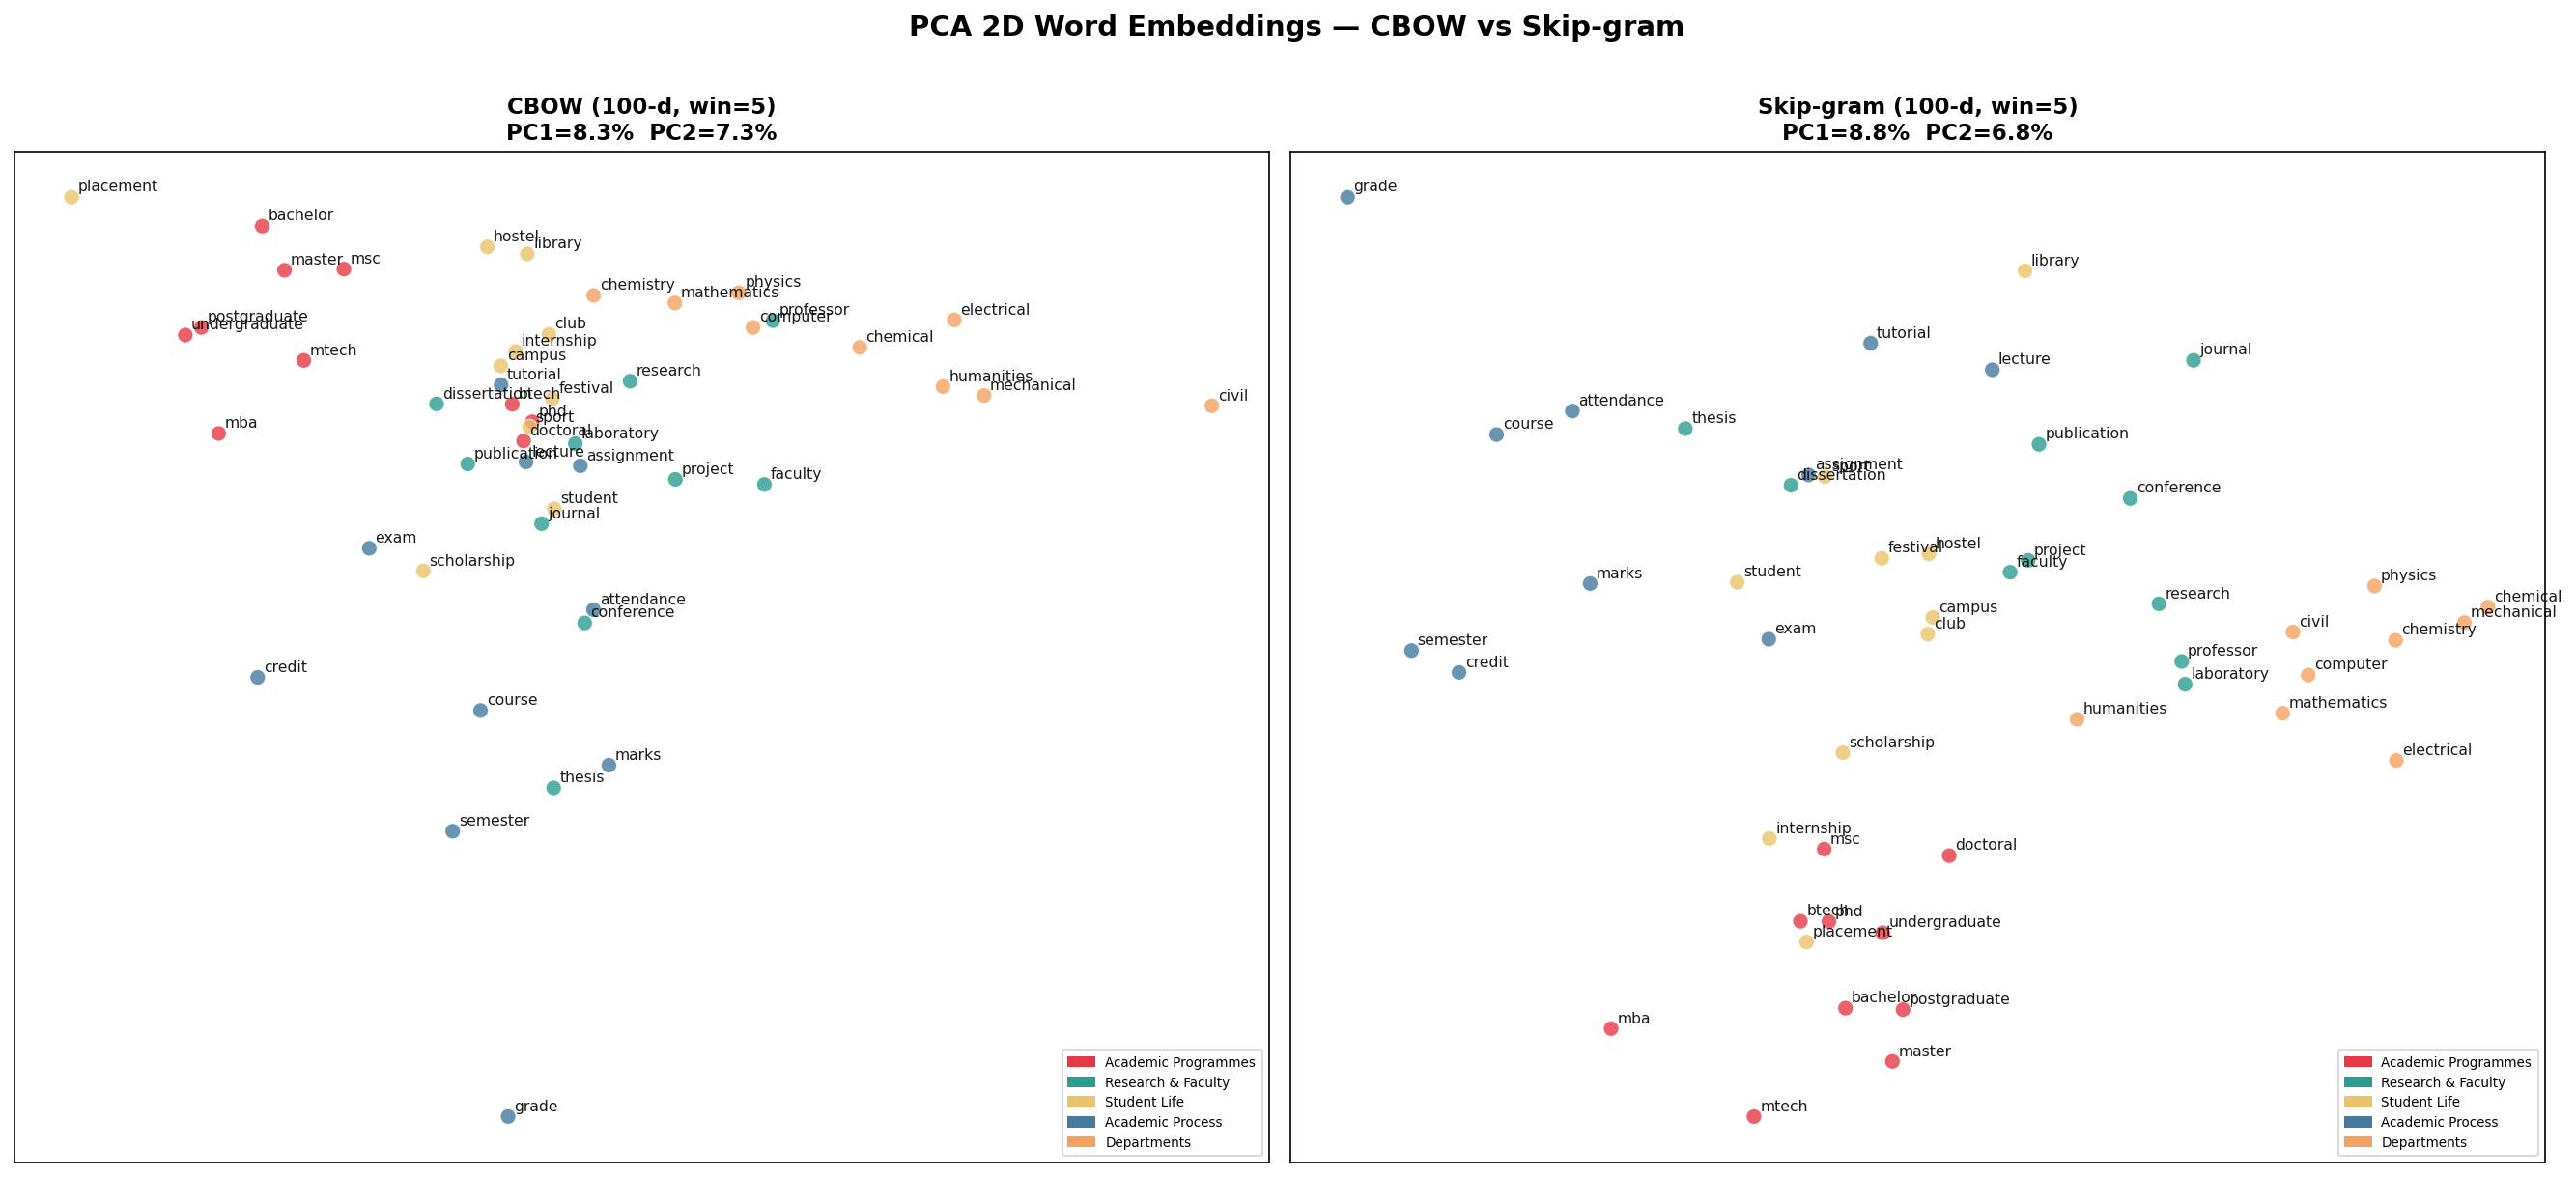
\includegraphics[width=\linewidth]{outputs/pca_cbow_vs_sgns.png}
  \caption{PCA 2D projection. Left: CBOW\_B; Right: SG\_B.}
  \label{fig:pca}
\end{figure}

In SG\_B, words from the same group (e.g.\ programme terms: \textit{doctoral, postgraduate, undergraduate}) cluster closer together, because Skip-gram gives sharper per-word representations. CBOW spreads things more evenly --- the context averaging dilutes distinctions.

\subsection{t-SNE Results}

\begin{figure}[H]
  \centering
  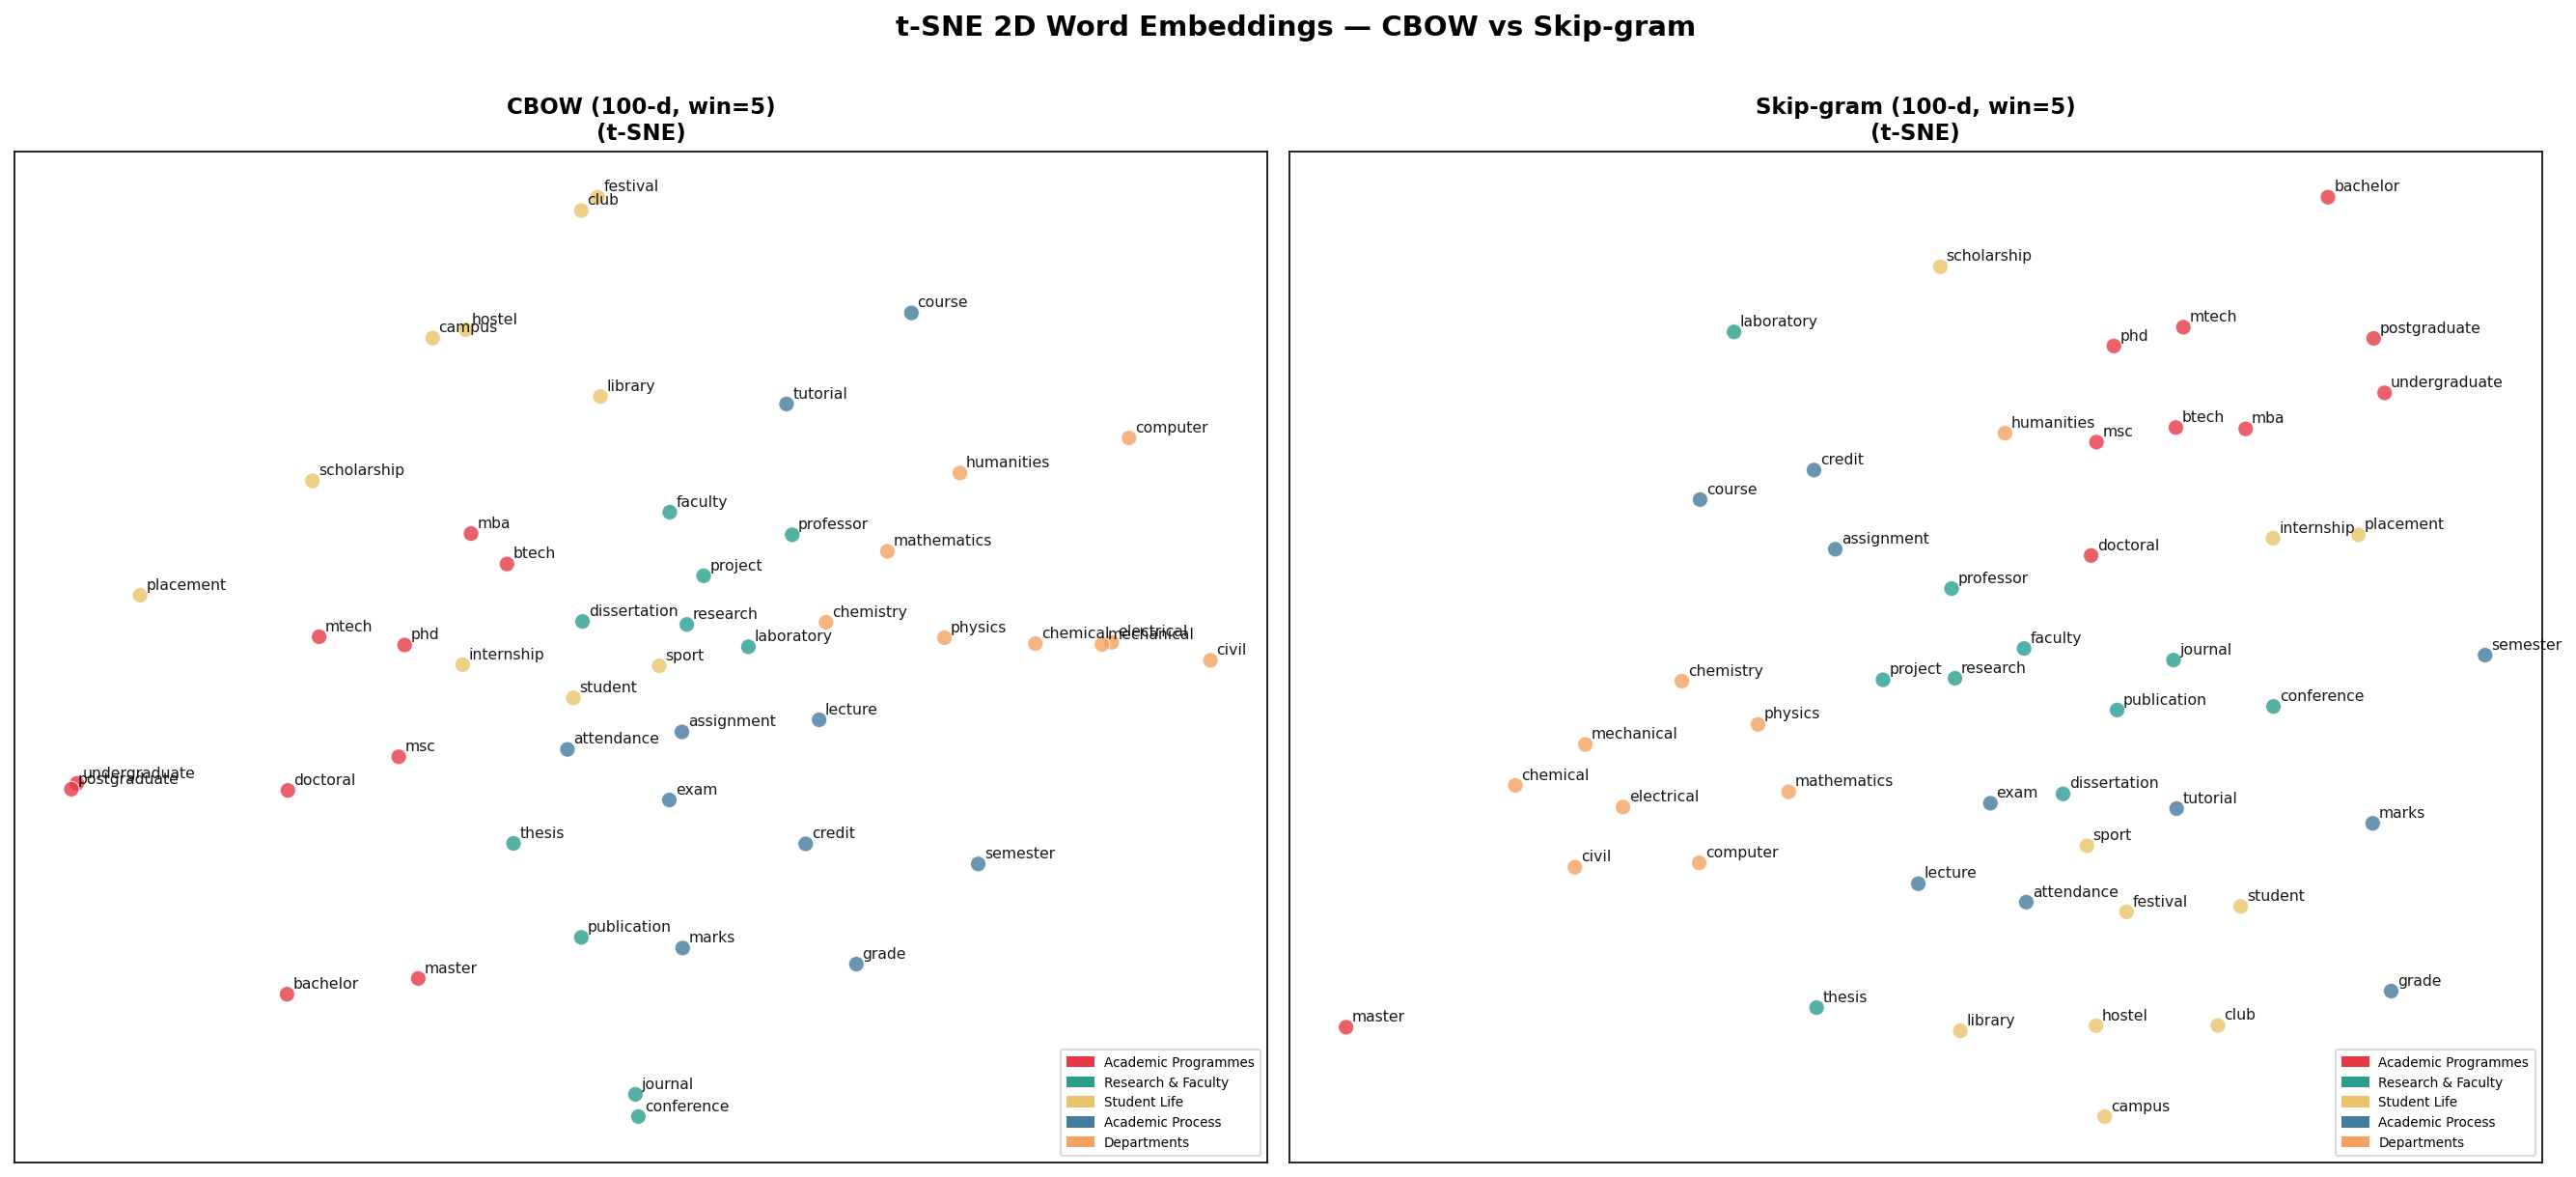
\includegraphics[width=\linewidth]{outputs/tsne_cbow_vs_sgns.png}
  \caption{t-SNE 2D projection (perplexity=10, 2000 iterations). Left: CBOW\_B; Right: SG\_B.}
  \label{fig:tsne}
\end{figure}

t-SNE reveals local structure more faithfully than PCA:

\begin{enumerate}[leftmargin=2em]
  \item \textbf{Skip-gram forms tighter semantic islands.} Research-lab terms cluster away from student-life terms much more clearly in SG\_B.
  \item \textbf{CBOW has a more spread-out layout.} Consistent with averaging: information is shared, making representations less distinguishable.
  \item Department names (\textit{computer, electrical, mechanical}) sit near Academic Programmes in both models --- makes sense since they share words like \textit{engineering, program, course}.
\end{enumerate}

% =========================================
\section{Conclusion}
% =========================================

\begin{enumerate}[leftmargin=2em]
  \item \textbf{Skip-gram beats CBOW for fine-grained semantics} on this corpus. It picks up specific academic terms much better (exam $\to$ syllabus/entrance vs.\ exam $\to$ thinkers/tuesday). But it's also more prone to noise (student names as phd neighbours).
  \item \textbf{The corpus works well.} 450K tokens from 51 source files (web pages + PDFs), vocab of 17K. The academic regulations PDFs alone gave us tons of semester/credit/thesis vocabulary.
  \item \textbf{Analogies partially work.} The ``semester : grade'' type analogies work because those terms co-occur in regulations text. Others fail due to corpus artifacts (concatenated tokens from PDF parsing).
  \item \textbf{Bigger dimensions help Skip-gram more.} SG\_C (200-d) makes tighter t-SNE clusters than SG\_A (50-d). For CBOW the difference is less obvious.
  \item \textbf{From-scratch vs.\ gensim.} Our numpy implementation is 64--136$\times$ slower (no C backend), and CBOW suffers from cosine saturation due to limited gradient updates per token. However, scratch Skip-gram (SG\_C) actually outperforms gensim on some analogies --- it correctly maps ``postgraduate'' $\to$ ``master'' while gensim returns a wrong answer. This shows that even a basic SGD loop can learn useful representations given enough dimensions and epochs.
  \item \textbf{Main limitation:} the corpus is admin-heavy (regulations, office pages, announcements). Adding course syllabi, lecture notes, or thesis abstracts would give richer academic embeddings.
\end{enumerate}

% --- references ---
\newpage
\section*{References}
\addcontentsline{toc}{section}{References}

\begin{enumerate}[leftmargin=2em, label={[\arabic*]}]
  \item Mikolov, T., Chen, K., Corrado, G., \& Dean, J.\ (2013). \textit{Efficient Estimation of Word Representations in Vector Space}. arXiv:1301.3781.
  \item Mikolov, T., Sutskever, I., Chen, K., Corrado, G., \& Dean, J.\ (2013). \textit{Distributed Representations of Words and Phrases and their Compositionality}. NeurIPS 2013.
  \item Firth, J.~R.\ (1957). \textit{A Synopsis of Linguistic Theory 1930--1955}. Studies in Linguistic Analysis.
  \item \v{R}eh\r{u}\v{r}ek, R.\ \& Sojka, P.\ (2010). \textit{Software Framework for Topic Modelling with Large Corpora}. LREC 2010. (Gensim library)
  \item van der Maaten, L.\ \& Hinton, G.\ (2008). \textit{Visualizing Data using t-SNE}. JMLR 9:2579--2605.
\end{enumerate}

\end{document}
